
\subsection{Armazenamento}

%%%%%%%%%%%%%%%%%%%%%%%%%%%%%%%%%%%	25	%%%%%%%%%%%%%%
%%%%%%%%%%%%%%%%%%%%%%%%%%%%%%%%%%%%%%%%%%%%%%%%%%%%%
\section{Banco de baterias}
\subsection*{Banco de baterias}
\begin{frame}{Banco de baterias}

\begin{figure}[H]
\includegraphics[scale=.32,center]{15}
\end{figure}

\end{frame}

%%%%%%%%%%%%%%%%%%%%%%%%%%%%%%%%%%%	26	%%%%%%%%%%%%%%
%%%%%%%%%%%%%%%%%%%%%%%%%%%%%%%%%%%%%%%%%%%%%%%%%%%%%
\begin{frame}{Banco de baterias}

\textbf{Número de baterias em série:}

\vspace{.25cm}
\centering

$N_S = \frac{V_{BANCO}}{V_{BAT}}$

\vspace{.25cm}

\justify
$N_S$ – Número de baterias ligadas em série

$V_{BANCO}$ – Tensão do banco de baterias [V]

$V_{BAT}$ – Tensão da bateria [V]

\end{frame}

%%%%%%%%%%%%%%%%%%%%%%%%%%%%%%%%%%%	27	%%%%%%%%%%%%%%
%%%%%%%%%%%%%%%%%%%%%%%%%%%%%%%%%%%%%%%%%%%%%%%%%%%%%

\begin{frame}{Banco de baterias}

\textbf{Energia armazenada no banco de baterias:}

\vspace{.25cm}
\centering

$E_A = \frac{E_C}{P_D} \quad [Wh]$
\vspace{.25cm}

\justify
$E_A$ – Energia armazenada no banco de baterias [Wh]

$E_C$ – Energia consumida [Wh]

$P_D$ – Profundidade de descarga permitida [\%]

\end{frame}

%%%%%%%%%%%%%%%%%%%%%%%%%%%%%%%%%%%	28	%%%%%%%%%%%%%%
%%%%%%%%%%%%%%%%%%%%%%%%%%%%%%%%%%%%%%%%%%%%%%%%%%%%%

\begin{frame}{Banco de baterias}

\textbf{Capacidade do banco de baterias:}

\vspace{.5cm}
\centering

$C_{BANCO} = \frac{E_A}{V_{BANCO}} \quad [Ah]$
\vspace{.25cm}

\justify
$C_{BANCO}$ – Capacidade de carga do banco de baterias [Ah]

$E_A$ – Energia armazenada no banco de baterias [Wh]

$V_{BANCO}$ – Tensão do banco de baterias [V]

\vspace{.25cm}
\begin{exampleblock}{}
\begin{center}
Geralmente são escolhidas baterias com capacidade mais próxima possível da capacidade total do banco.
\end{center} 
\end{exampleblock}

\end{frame}

%%%%%%%%%%%%%%%%%%%%%%%%%%%%%%%%%%%	29	%%%%%%%%%%%%%%
%%%%%%%%%%%%%%%%%%%%%%%%%%%%%%%%%%%%%%%%%%%%%%%%%%%%%
\begin{frame}{Banco de baterias}

\textbf{Número de baterias em paralelo:}

\vspace{.25cm}
\centering

$N_{BP} = \frac{C_{BANCO}}{C_{BAT}}$
\vspace{.25cm}

\justify
$N_{BP}$ – Número de conjuntos de baterias ligadas em paralelo

$C_{BANCO}$ – Capacidade de carga do do banco de baterias [Ah]

$C_{BAT}$ – Capacidade de carga de cada bateria [Ah]

\end{frame}

%%%%%%%%%%%%%%%%%%%%%%%%%%%%%%%%%%%%	30	%%%%%%%%%%%%%%
%%%%%%%%%%%%%%%%%%%%%%%%%%%%%%%%%%%%%%%%%%%%%%%%%%%%%%
%\section{Inversores}
%\subsection*{Inversores}
%\begin{frame}{Inversores}
%
%\textbf{Operação}
%\begin{itemize}
%\item Funciona unicamente quando está conecto à rede elétrica
%
%\item Possui um esquema anti-ilhamento (segurança)
%\end{itemize}
% 
%\begin{figure}[H]
%\includegraphics[scale=.28,center]{16}
%\end{figure}
%
%\end{frame}
%
%%%%%%%%%%%%%%%%%%%%%%%%%%%%%%%%%%%%	31	%%%%%%%%%%%%%%
%%%%%%%%%%%%%%%%%%%%%%%%%%%%%%%%%%%%%%%%%%%%%%%%%%%%%%
%
%\begin{frame}{Inversores}
%
%\begin{columns}[T]
%    \begin{column}{0.5\textwidth}
%    \vspace{.5cm}
%    	\textbf{Características}
%    \end{column}
%    \begin{column}{0.5\textwidth}
%    	\centering
%      	\includegraphics[scale=.2,right]{17}
%    \end{column}
%\end{columns}
% 
%\begin{figure}[H]
%\includegraphics[scale=.33,center]{18}
%\end{figure}
%
%\end{frame}
%
%%%%%%%%%%%%%%%%%%%%%%%%%%%%%%%%%%%%	32	%%%%%%%%%%%%%%
%%%%%%%%%%%%%%%%%%%%%%%%%%%%%%%%%%%%%%%%%%%%%%%%%%%%%%
%\begin{frame}{Inversores}
%
%\begin{columns}[T]
%    \begin{column}{0.5\textwidth}
%    \vspace{.5cm}
%    	\textbf{Características}
%    \end{column}
%    \begin{column}{0.5\textwidth}
%    	\centering
%      	\includegraphics[scale=.2,right]{19}
%    \end{column}
%\end{columns}
% 
%\begin{figure}[H]
%\includegraphics[scale=.33,center]{20}
%\end{figure}
%
%\end{frame}
%
%%%%%%%%%%%%%%%%%%%%%%%%%%%%%%%%%%%%	33	%%%%%%%%%%%%%%
%%%%%%%%%%%%%%%%%%%%%%%%%%%%%%%%%%%%%%%%%%%%%%%%%%%%%%
%\section{Medidor Bidirecional}
%\subsection*{Medidor Bidirecional de Energia}
%\begin{frame}{Medidor Bidirecional de Energia}
%
%Indica o sentido de fluxo da energia
%
%\vspace{.35cm}
%\centering
%{\Large fonte <=> carga}
%
%\vspace{.35cm}
%
%\begin{columns}[T]
%    \begin{column}{0.5\textwidth}
%    	\centering
%      	\includegraphics[scale=.35,center]{21}
%    \end{column}
%    \begin{column}{0.5\textwidth}
%    	\centering
%      	\includegraphics[scale=.45,center]{22}
%    \end{column}
%\end{columns}
% 
%\end{frame}
%
%%%%%%%%%%%%%%%%%%%%%%%%%%%%%%%%%%%%	34	%%%%%%%%%%%%%%
%%%%%%%%%%%%%%%%%%%%%%%%%%%%%%%%%%%%%%%%%%%%%%%%%%%%%%
%\begin{frame}{Medidor Bidirecional de Energia}
%
%O gráfico a seguir indica os quatro quadrantes de acordo com os valores de energia
%
%\begin{figure}[H]
%\includegraphics[scale=.45,center]{23}
%\end{figure}
%
%\vspace{-.5cm}
%\begin{figure}[H]
%\includegraphics[scale=.45,center]{24}
%\end{figure}
%
%\end{frame}
%
%%%%%%%%%%%%%%%%%%%%%%%%%%%%%%%%%%%%	35	%%%%%%%%%%%%%%
%%%%%%%%%%%%%%%%%%%%%%%%%%%%%%%%%%%%%%%%%%%%%%%%%%%%%%
%\section{Exemplo}
%\subsection*{Exemplo}


%\begin{frame}{Exemplo}
%
%Dimensionar um sistema fotovoltaico para atender o consumo diário de um pequeno escritório que possui os seguintes aparelhos
%
%\begin{itemize}
%\item Lâmpada fluorescente compacta - 11 w
%\item Modem de internet
%\item Roteador
%\item Impressora 
%\end{itemize}
%
%\end{frame}
%%%%%%%%%%%%%%%%%%%%%%%%%%%%%%%%%%%%	36	%%%%%%%%%%%%%%
%%%%%%%%%%%%%%%%%%%%%%%%%%%%%%%%%%%%%%%%%%%%%%%%%%%%%%%
%\begin{frame}{Exemplo}
%
%\textbf{Condições do sistema
%}
%
%\begin{itemize}
%\item Baterias de chumbo ácido de 12 Vcc
%\item Tensão do banco de baterias de 24 Vcc
%\item Descarga máxima de 50%
%\item Controlador de carga convencional
%\item Capacidade de armazenamento para dois dias
%\item Módulos Solares Bosch c-Si M 60 – Designação 250
%\item Tensão da instalação elétrica 127 Vac
%\end{itemize}
%
%\end{frame}
%
%%%%%%%%%%%%%%%%%%%%%%%%%%%%%%%%%%%%	37	%%%%%%%%%%%%%%
%%%%%%%%%%%%%%%%%%%%%%%%%%%%%%%%%%%%%%%%%%%%%%%%%%%%%%%
%\begin{frame}{Exemplo}
%
%\textbf{Organização do sistema
%}
%
%\begin{itemize}
%\item Quatro baterias de 240 Ah / 24V
%\item Cinco módulos solares Bosch c-Si M 60 – Designação 250
%\item Um controlador de carga 24 V / 60 A
%\item Um inversor 24 Vcc / 127 Vac
%
%\end{itemize}
%
%\end{frame}



\begin{frame}{Dúvidas?}

\end{frame}


%%%%%%%%%%%%%%%%%%%%%%%%%%%%%%%%%%%%%%%%%%%%%%%%%%%%%%
%%%%%%%%%%%%%%%%%%%%%%%%%%%%%%%%%%%%%%%%%%%%%%%%%%%%%%%
%\begin{frame}{}
%
%\begin{figure}[H]
%		\includegraphics[scale=.55,center]{formulas}
%\end{figure}
%
%\end{frame}
%%----------------------->
%\subsection{Tipos de SFV}
%%----------------------->
%
%\begin{frame}{Tipos de SFV}
%
%Também se faz necessário saber que tipo de SFV está sendo projetado
%
%\vspace{.5cm}
%
%\begin{itemize}
%\item Conectado à rede (On-Grid)
%\item Autónomo, Isolado ou Independente (Off-Grid)
%\end{itemize}
%
%\begin{figure}[H]
%	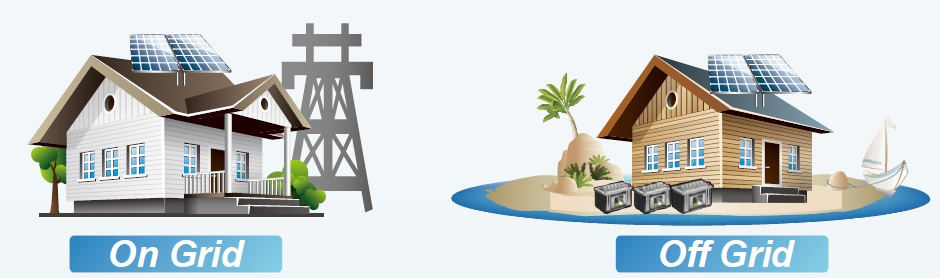
\includegraphics[scale=.4,center]{on-off-grid-solar-power-system}
%\end{figure} 
%
%\end{frame}
%
%%----------------------->
%\section{Componentes}
%\subsection{Componentes}
%%----------------------->
%
\begin{frame}{Componentes dos SFV}

Os SFV são altamente customizáveis, eles podem ser projetados para operar em determinados períodos de tempo ou de acordo com a necessidade de consumo do local.

\begin{center}
    \resizebox{0.6 \linewidth}{!}{%
\begin{tikzpicture}[node distance = 2cm, auto]

\node[Med_block]					(ppv) {Arranjo\\ Fotovoltaico};
\node[Big_esp_block, right=1cm of ppv]	(uccp) {Unidade de Controle\\ e Acondicionamento\\ de Potência};
\node[Med_block, right=1cm of uccp]	(carg) {Carga};
\node[Med_block, above=1cm of carg]	(arma) {Armazena-\\ mento};
\node[Med_block, below=1cm of carg]	(rede) {Rede\\ Elétrica};

\path[line] (ppv) -- (uccp);
\path[line] (uccp) -- (carg);
\path[line] (uccp) -- (arma);
\path[line] (uccp) -- (rede);
 \end{tikzpicture}
    }%
\end{center}
 
\begin{exampleblock}{}
	\begin{center}
	A capacidade para personalizar cada instalação ajuda a minimizar os custos do projeto 
	\end{center} 
\end{exampleblock}
 
 
\end{frame}

%\begin{frame}{viabilidade}
%
%Os fatores que afetam a viabilidade de um projeto de de Sistema Fotovoltaico (SFV) são listados a seguir:
%
%\begin{itemize}
%\item Local
%	\begin{itemize}
%	\item Acesso à rede elétrica
%	\item Terreno e espaço (telhados, áreas abertas e planas)
%	\end{itemize}
%\item Recurso energético
%	\begin{itemize}
%	\item Radiação solar direta (disponibilidade >75\% do ano) 
%	\end{itemize} 
%\item Benefícios financeiros 	\begin{itemize}
%	\item Investimento inicial (aquisição e instalação de equipamentos)
%	\item Custos de Operação e Manutenção
%	\item Tarifa da energia elétrica
%	\item Impostos ou incentivos
%	\item Taxas de correção e Tempo de retorno
%	\end{itemize}
%\end{itemize}
%
%\begin{exampleblock}{}
%	\begin{center}
%	Certifique-se de considerar os desafios de hoje e do futuro
%	\end{center} 
%\end{exampleblock}
%
%\end{frame}
%
\begin{frame}{Componentes dos SFV}

Sistema On-Grid

\begin{center}
    \resizebox{0.9 \linewidth}{!}{%
\begin{tikzpicture}[node distance = 2cm, auto]

\node[Med_block]					(ppv) {Arranjo\\ Fotovoltaico};
\node[Med_esp_block, right=1cm of ppv]	(inv) {Inversor};
\node[Med_esp_block, right=1cm of inv]	(qua) {Quadro de\\ Controle};
\node[Med_block, right=1cm of qua]	(med) {Medição\\ Bidirecional};
\node[Med_block, right=1cm of med](red) {Rede\\ Elétrica};
\node[Med_block, below=1cm of qua](car) {Carga\\ AC};

\path[line] (ppv) -- (inv);
\path[line] (inv) -- (qua);
\path[line] (qua) -- (med);
\path[line] (med) -- (red);
\path[line] (red) -- (med);
\path[line] (qua) -- (car); 
 \end{tikzpicture}
    }%
\end{center}

Sistema Off-Grid

\begin{center}
    \resizebox{0.7 \linewidth}{!}{%
\begin{tikzpicture}[node distance = 2cm, auto]

\node[Med_block]					(ppv) {Arranjo\\ Fotovoltaico};
\node[Med_esp_block, right=1cm of ppv]	(con) {Controlador\\ de Carga};
\node[Med_block, right=1cm of con]	(inv) {Inversor};
\node[Med_block, right=1cm of inv](cca) {Carga\\ CA};
\node[Med_block, below=1cm of con]	(bat) {Bateria};
\node[Med_block, right=1cm of bat](ccc) {Carga\\ CC};

\path[line] (ppv) -- (con);
\path[line] (con) -- (inv);
\path[line] (inv) -- (cca);
\path[line] (con) -- (bat);
\path[line] (con) -- (ccc);
 \end{tikzpicture}
    }%
\end{center}
 
\end{frame}

%%\textbf{Exemplo:} 1.2 kWh/m2/dia (Média anual) obtidos do mapa Solarimétrico para certa localidade.
%%\textbf{Interpretação:} Soma da irradiação de cada dia do ano dividida por 365
